\section{Module 2: Lecture 7\\Fourier Transforms properties and Fourier series example}

\subsection{Introduction}
	In this section, we will take a few examples of the calculation of the Fourier transform and then build upon the general properties of a Fourier transform like linearity, time shift, modulation and convolution. \\
	Let us start with calculating the Fourier transform of a rectangular pulse.
\subsection{Fourier transform of a Rectangular Pulse}
	Let the pulse be symmetric, with height equal to $A$, going from $-T/2$ to $T/2$ on the time axis. We call this function $h(t)$ as shown in Fig.\ref{fig:rectangular_pulse}.
	%%%
	\begin{figure}[htp]
		\centering
		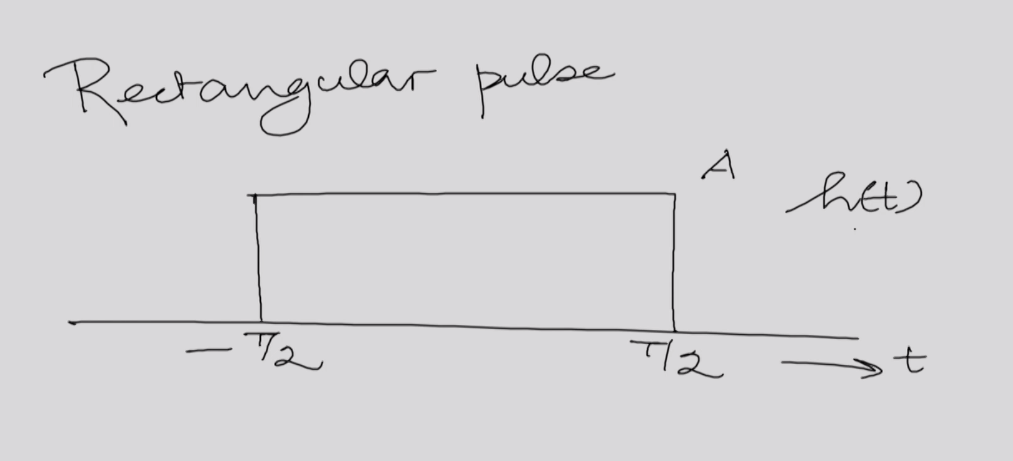
\includegraphics[width=12cm]{rectangularpulse.png}
		\caption{Symmetric Rectangular Pulse}
		\label{fig:rectangular_pulse}
	\end{figure}
	%%%
	Let us denote the Fourier transform by $ H(\Omega)$. Then
	\begin{equation}
		H(\Omega)=\int_{-\infty}^{\infty} \! {h(t) e^{-j\Omega t}} \ \dm t
	\end{equation}
	As $h(t)$ is zero except in the time interval $-T/2$ to $T/2$, we can write the above equation as
	\begin{equation}
		H(\Omega)=\int_{-T/2}^{T/2} \! {A e^{-j\Omega t}} \ \dm t =
		\frac{A e^{-j\Omega t}}{-j \Omega} \Bigg|_{-T/2}^{T/2}=
		\frac{A(e^{-j\Omega T/2}-e^{j\Omega T/2})}{-j\Omega}
		=\frac{AT (2j\sin({\Omega T/2}))}{j\Omega T}
	\end{equation}

	\begin{equation}
		H(\Omega)=\frac{AT\sin({\Omega T/2})}{\Omega T/2}
	\end{equation}
	And we can rewrite it as

	\begin{equation}
		H(f)=\frac{AT \sin({2\pi f T/2})}{2\pi f T/2}
	\end{equation}
	Where $f = \cfrac{\Omega}{2\pi}$ corresponds to the ${cycles}/{second}$ frequency, and $\Omega$ is of course the angular frequency.
	Now this expression also can be written as
	\begin{equation}
		H(\gamma)=\frac{AT \sin({\pi \gamma})}{\pi \gamma}
	\end{equation}
	Where $\gamma = f*T $.\\
	The function $\cfrac{\sin{\pi \gamma}}{\pi \gamma}$ is a very special function called a \emph{Sinc Function}. The sinc function in the form presented is often used in the context of signals and systems.

	\subsubsection{Sketch of the Sinc function}

		Here are the some properties of the Sinc function.
		\begin{itemize}
			\item It is an even function.
			\item It has nulls at every integer; so at 1, at 2, at 3 and so on, it will have value equal to zero.
			\item It tends to 1 as $\gamma$ tends to 0
			\item It is a damped sinusoid, i.e. the magnitude of oscillation decreases as $\gamma$ increases.
		\end{itemize}
		Using the above points we can sketch the Sinc function. So the sketch somewhat looks like Fig\ref{fig:sinc}.
		\begin{figure}[htp]
			\centering
			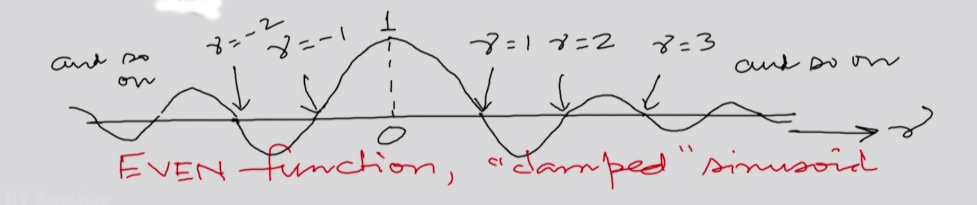
\includegraphics[width=12cm]{sinc.png}
			\caption{Sinc Function}
			\label{fig:sinc}
		\end{figure}

	\subsubsection{Important points regarding the Fourier transform of rectangular pulse}
		The pulse is limited in terms of its occupancy of the time axis. It goes only from  $-T/2$ to $+T/2$. On the other hand, the Fourier transform, in principle, lasts all over the frequency axis.
		What this means is that if we want to make a function vanish all over the time axis outside a certain finite interval, we have to bring together frequencies of all magnitudes and signs except for a few nulls.
		All these frequencies need to come together, in appropriate amplitudes, to form this rectangular pulse. Also note that the Fourier transform for this case is purely real. \\
		 When the pulse width is halved, the nulls of the Fourier transform are doubly spaced and the central amplitude is halved. This can be checked mathematically. We can see that Fig\ref{fig:pulse_FT_half}.
		\begin{figure}[htp]
			\centering
			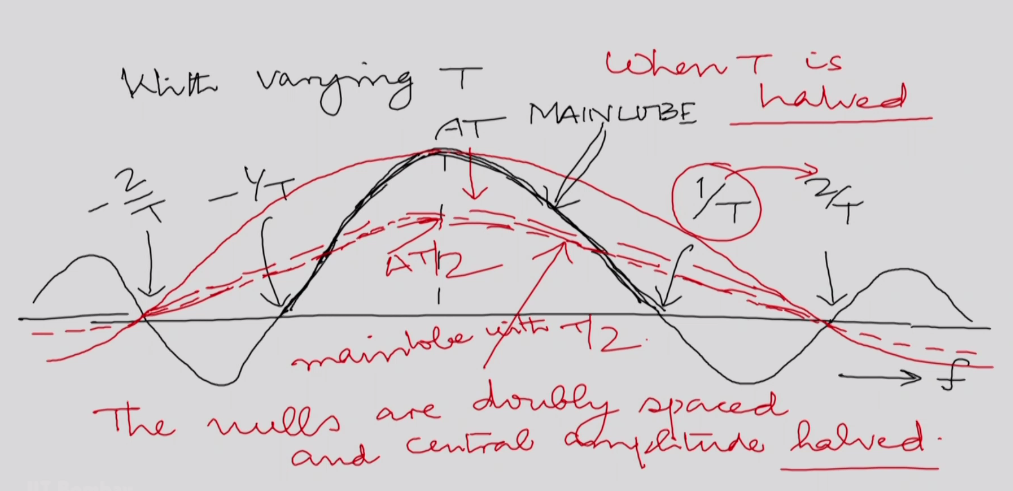
\includegraphics[width=12cm]{pulse_FT_half.png}
			\caption{Fourier Transform of Rectangular Pulse at width T and T/2 }
			\label{fig:pulse_FT_half}
		\end{figure}

\subsection{Properties of Fourier Transform}
	Let us see what happens to the Fourier transform when we change the original signal in some particular way.
	% When we change the signal in some way or when we bring signals together, what happens to the corresponding Fourier transform is what we will investigate in this section.
	\subsubsection{Linearity}
		Let $h_1(t)$ have the Fourier transform $H_1(\Omega)$ and let $h_2(t)$ have the Fourier transform $H_2(\Omega)$. Then, linearity says

		%\begin{equation}
		%$$\alpha h_1(t) + \beta h_2(t) \longrightarrow \alpha H_1(\Omega)+ \beta H_2(\Omega)$$
		%\end{equation}


		\[\alpha h_1(t) + \beta h_2(t) \xrightarrow{\mathcal{F}} \alpha H_1(\Omega)+ \beta H_2(\Omega)\]
		for all $\alpha$, $\beta$ $\in \mathbb{C}$ and all $h_1(t)$ and $h_2(t)$. Here, ${\mathcal{F}}$ means ``has the Fourier transform given by".

	\subsubsection{Proof of linearity}
		\begin{equation}
			 \alpha \{ H_1(\Omega) \} = \alpha \{ \int_{-\infty}^{\infty} \! h_1(t)e^{-j\Omega t} \ \dm t \}
			\label{eqn:one}
		\end{equation}

		\begin{equation}
			 \beta \{ H_2(\Omega) \} = \beta \{ \int_{-\infty}^{\infty} \! h_2(t)e^{-j\Omega t} \ \dm t \}
			\label{eqn:two}
		\end{equation}
		Add Eqn.\ref{eqn:one} and \ref{eqn:two}. We can write it as
		\begin{equation}
			\{ \alpha H_1(\Omega) + \beta H_2(\Omega) \} = \{ \int_{-\infty}^{\infty} \! (\alpha h_1(t) + \beta h_2(t))e^{-j\Omega t} \ \dm t \}
		\end{equation}

	\subsubsection{The Inverse Fourier transform}
		THe Inverse Fourier transform can be written as
		\begin{equation}
			H_1(\Omega) \xrightarrow{\mathcal{F}^{-1}} \frac{1}{2\pi} \int_{-\infty}^{\infty} \! H_1(t) e^{j\Omega t} \ \dm \Omega
		\end{equation}
		Note that $\Omega$ = $2\pi f$ and $d\Omega$= $2\pi df$. Hence,
		%%%
		\begin{equation}
			H_1(f) \xrightarrow{\mathcal{F^-1}} \int_{-\infty}^{\infty} \! H_1(f) e^{j2\pi ft} \ \dm f
		\end{equation}
		%%%
		Where $\Omega$ =  Radians/sec frequency
		And $f$ = cycles/sec frequency
		%%%
		\begin{itemize}
			\item We can clearly see that when frequency is in radians/sec then, we will have factor of $1/2\pi$ in the inverse Fourier transform and when frequency is in cycles/sec then the factor of $1/2\pi$ will not be there.
			\item In a way dealing with cycles/second frequency has some conveniences; we don't need to remember the factor of $1/2\pi$, or we can say, there is a perfect symmetry between the Fourier transform and the Inverse Fourier transform.
		\end{itemize}

	\subsubsection{Exercise}
		 Prove that linearity holds true for the inverse Fourier transform.

\subsection{Time Shift}
	What happens to the Fourier transform when we shift the signal in time? If
	\begin{equation}
		h(t) \xrightarrow{\mathcal{F}} H(\Omega)
	\end{equation}
	then, for a constant $\tau$,
	\begin{equation}
		h(t-\tau) \xrightarrow{\mathcal{F}} {?}
	\end{equation}
	%%%
	The Fourier transform would be
	\begin{equation}
		H(\Omega) =  \int_{-\infty}^{\infty} \! h(t-\tau) e^{-j\Omega t} \ \dm t
	\end{equation}
	Put $(t-\tau) = \lambda$  $\Rightarrow$  $t = \tau + \lambda$.
	So the Fourier transform is
	\begin{equation}
		H(\Omega) =  \int_{-\infty}^{\infty} \! h(\lambda) e^{-j\Omega (\lambda + \tau)} \ \dm \lambda =
		e^{-j\Omega \tau} \int_{-\infty}^{\infty} \! h(\lambda) e^{-j\Omega \lambda} \ \dm \lambda
	\end{equation}
	So,
	\begin{equation}
		h(t-\tau) \xrightarrow{\mathcal{F}} e^{-j\Omega \tau} H(\Omega)\   or\   e^{-j2\pi f\tau} H(f)
	\end{equation}
	Now it can be clearly seen that
	\begin{itemize}
		\item The magnitude of the Fourier transform is unchanged.
		\item The angle or the phase of the Fourier transform changes.
	\end{itemize}

	\subsubsection{Modulation}
		By modulation, we mean multiplying $h(t)$ by a rotating complex number (rotating with an angular velocity of $\Omega_0$). In this case, the Fourier transform is shifted by $\Omega_0$ forward.

		\begin{equation}
			e^{j\Omega_0 t} h(t) \xrightarrow{\mathcal{F}} {?}
		\end{equation}
		So the Fourier transform would be
		\begin{equation}
			 \int_{-\infty}^{\infty} \! e^{j\Omega_0 t} h(t) e^{-j\Omega t} \ \dm t =
			 \int_{-\infty}^{\infty} \! h(t) e^{-j(\Omega-\Omega_0) t} \ \dm t =
			 H(\Omega-\Omega_0)
		\end{equation}
		
		\begin{itemize}
			\item When we shift a function in time, it causes a modulation in the frequency domain (We remember, it multiplied the Fourier transform by a term $e^{-j\Omega \tau_0}$).

			\item When we modulate the function in time by multiplying by a rotating complex number, the corresponding Fourier transform shifts in frequency.

			\item Basically, shift in time becomes modulation in frequency, and modulation in time becomes a shift in frequency.
		\end{itemize}

	\subsubsection{Convolution Property of Fourier transform}
		The question to answer here is what will be the Fourier transform of $x_1(t)*x_2(t)$, given that the Fourier transforms of $x_1(t)$ and $x_2(t)$ are $X_1(\Omega)$ and $X_2(\Omega)$ respectively. 

		\begin{equation}
			x_1(t)\ast x_2(t) = \int_{-\infty}^{\infty}{x_1(\tau) x_2(t-\tau)}d\tau
		\end{equation}

		\begin{equation}
			x_1(t)\ast x_2(t) \xrightarrow{\mathcal{F}} {?}
		\end{equation}
		\noindent
		Now let's solve it. The Fourier transform can be written as
		\begin{equation}
			\int_{-\infty}^{\infty} \! \{ \int_{-\infty}^{\infty} \! x_1(\tau) x_2(t-\tau) \ \dm \tau \} e^{-j\Omega t} \ \dm t
		\end{equation}
		This is same as
		\begin{equation}
			\int_{-\infty}^{\infty} \! \int_{-\infty}^{\infty} \! x_1(\tau) x_2(t-\tau) e^{-j\Omega t} \ \dm \tau \dm t
		\end{equation}
		To solve the above double integral we will do a change of variables. Put
		\begin{equation}
			\alpha =\tau \ \text{and} \ \beta = (t-\tau)
		\end{equation}

		\begin{equation}
			\left( \begin{array}{c}
			\alpha \\
			\beta \end{array} \right)
			=
			\left( \begin{array}{cc}
			1 & 0 \\
			-1 & 1 \end{array} \right)
			\left( \begin{array}{c}
			\tau \\
			 t \end{array} \right)
		\end{equation}

		\begin{equation}
			\mathrm{d}\tau \mathrm{d}t = |\text{Det(transformation)}| \mathrm{d}\alpha \mathrm{d}\beta
		\end{equation}
		\noindent
		Hence,
		\begin{equation}
			\mathrm{d}\tau \mathrm{d}t = \mathrm{d}\alpha \mathrm{d}\beta
		\end{equation}
		Hence, the element of integration also remains the same because the Jacobian is $1$. Now the modified integral is
		
		\begin{equation}
			\int_{-\infty}^{\infty} \! \int_{-\infty}^{\infty} \! x_1(\alpha) x_2(\beta) \exp{-j\Omega(\alpha+\beta)} \ \dm \alpha \dm \beta
		\end{equation}
		
		\begin{equation}
			=\int_{-\infty}^{\infty} \! x_1(\alpha) \{ \int_{-\infty}^{\infty} \!
			x_2(\beta) e^{-j\Omega(\beta)} \ \dm \beta \} e^{-j\Omega \alpha} \ \dm \alpha
		\end{equation}
		This can be written as
		
		\begin{equation}
			X_2(\Omega) \int_{-\infty}^{\infty} \! x_1(\alpha) e^{-j\Omega \alpha} \ \dm \alpha
		\end{equation}
		So
		\begin{equation}
			x_1(t) \ast x_2(t) \xrightarrow{\mathcal{F}} X_1(\Omega)X_2(\Omega)
		\end{equation}
		\noindent
		Hence a convolution in the natural domain becomes a multiplication in the Fourier domain.

\subsection {Conclusion} In this section, we discussed about the Fourier transform of a rectangular pulse which is the ``Sinc function'', and its properties. We showed some of the properties of Fourier transform and their proofs.